This chapter describes the collision data and simulated event samples used for searching electroweak production of SUSY states in compressed scenarios.
The collision data are presented in Sect.~\ref{sec:data_collision_data} and the Monte Carlo (MC) simulated event samples are detailed in Sect.~\ref{sec:data_MC_samples}.
%The samples used for searching the strongly-produced SUSY particles in final states with two same-sign or three lepton and jets (SS/3L+jets) can be found in the App.~\ref{sec:app_samples_strong}.


\section{Collision data}
\label{sec:data_collision_data}
The LHC $pp$ collision data used in this analysis were collected by the ATLAS detector at $\sqrt{s} = 13$~{\TeV} during 2015 and 2016.
The data corresponds to an integrated luminosity of 36.1~{\ifb} (3.2~{\ifb} in 2015 and 32.9~{\ifb} in 2016) with a combined uncertainty of 2.1\% after applying beam, detector, and data-quality requirements.
The combined uncertainty is derived following the methodology similar to those described in Ref.~\cite{Aaboud:2016hhf}.
The average number of $pp$ interactions per bunch crossing (pileup) is 13.5 in the 2015 data set and is 25 in the 2016 data set.
The data samples are required to satisfy the following good runs list (GRLs) as recommended by the ATLAS collaboration
%
\begin{itemize}
    \item \texttt{data15\_13TeV.periodAllYear\_DetStatus-v79-repro20-02\_DQDefects\\-00-02-02\_PHYS\_StandardGRL\_All\_Good\_25ns.xml}
    \item \texttt{data16\_13TeV.periodAllYear\_DetStatus-v88-pro20-21\_DQDefects\\-00-02-04\_PHYS\_StandardGRL\_All\_Good\_25ns.xml}
\end{itemize}
%
Events are selected using different inclusive \met triggers depending on the run period as listed in Table.~\ref{tab:data_triggers}.
Two new triggers, \texttt{HLT\_mu4\_j125\_xe90\_mht} and \texttt{HLT\_2mu4\_j85\_xe50\_mht}\footnote{\texttt{HLT\_mu4\_j125\_xe90\_mht} means high level trigger with $\pt(\mu) > 4$, $\pt(\mathrm{jets}) > 125$, and $\met > 90$~{\GeV} and \texttt{HLT\_2mu4\_j85\_xe50\_mht} means high level trigger two muons with $\pt > 4$, $\pt(\mathrm{jets}) > 85$, and $\met > 50$~{\GeV}.}, are developed for compressed scenarios starting from run number 308084.
However, these new triggers only contribute a small gain compared to the inclusive \met triggers.
This analysis uses inclusive \met triggers only.

\begin{table}[htp]
    \begin{center}
        {\footnotesize
            \begin{tabular}{ll}
                \hline
                \hline
                Run period & \met trigger\\
                \hline
                2015 & \texttt{HLT\_xe70\_mht}\\
                A-D3 & \texttt{HLT\_xe90\_mht\_L1XE50}\\
                D4-F1 & \texttt{HLT\_xe100\_mht\_L1XE50}\\
                F1- & \texttt{HLT\_xe110\_mht\_L1XE50}\\
                \hline
                \hline
            \end{tabular}
        }
    \end{center}
    \caption{The inclusive \met triggers used in this analysis.
    The \met threshold varies from 70 (xe70) to 110 (xe110)~{\GeV} depending on the run period.
    The trigger naming convention and definition can be found at~\cite{ATLAS:twiki_trigger}.}
    \label{tab:data_triggers}
\end{table}%

%%%
%%%
%%%

\section{Monte Carlo simulated event samples}
\label{sec:data_MC_samples}
MC samples are used to model the SUSY signals and to estimate the SM background.
All SM background MC samples were processed through a detailed ATLAS detector simulation based on {\GEANT}4~\cite{Agostinelli:2002hh} and the SUSY signal samples were simulated by a fast simulation (AF2) that parameterizes the calorimeter response~\cite{ATLAS:2010bfa}.
To simulate the effects of additional $pp$ collisions (pileup) in the same and nearby bunch crossings, inelastic interactions were generated using the soft QCD processes of {\PYTHIA} v8.186~\cite{Sjostrand:2007gs} with A2 tune~\cite{ATLAS:2012uec} and the MSTW2008LO PDF set~\cite{Martin:2009iq}.
These MC events were overlaid onto each simulated hard-scatter event and reweighted to match the pileup conditions observed in the data.

%%%
%%%
%%%

\subsection{The SM background samples}
\label{subsec:data_sm_bkg_samples}
Table~\ref{tab:data_mc_samples} summarizes the event generator configurations of the ME, parton shower (PS), PDF set, and the cross-section normalization.
The {\SHERPA} 2.1.1, 2.2.1, and 2.2.2 ~\cite{Gleisberg:2008ta} were used to produce the $Z^{(*)}/\gamma^{*}$ + jets, diboson, and triboson events.
The matrix elements (ME) were calculated for up to two partons at next-to-leading order (NLO) and up to four partons at leading order (LO) depending on the process.
The $Z^{(*)}/\gamma^{*}$ + jets and diboson samples cover the dilepton invariant masses from 0.5~{\GeV} for $Z^{(*)}/\gamma^{*} \to e^{+}e^{-}/\mu^{+}\mu^{-}$ and from 3.8~{\GeV} for $Z^{(*)}/\gamma^{*} \to \tau^{+}\tau^{-}$.
{\POWHEG}-Box v1 and v2 interfaced to {\PYTHIA} 6.428 were used to simulated \ttbar and single-top production at NLO in the ME.
The Higgs boson production were generated using {\POWHEG}-Box v2 interfaced to {\PYTHIA} 8.186.
A Higgs boson in association with a $W$ or $Z$ boson production was simulated using MG5\_{\scriptsize A}MC@NLO 2.2.2 with {\PYTHIA} 8.186 and the ATLAS A14 tune.
The processes containing \ttbar and at least one electroweak bosons were produced using MG5\_{\scriptsize A}MC@NLO 2.2.1, 2.2.2, 2.3.2, 2.3.3 with {\PYTHIA} 6.4.28 or 8.186.
These processes were generated at NLO in the ME except for $t + Z$ and $t +$ \ttbar which were produced at LO.
Except those produced by {\SHERPA} event generator, the \textsc{EvtGEN}\xspace v1.2.0~\cite{Lange:2001uf} was used to model the decay of bottom and charm hadrons in all MC samples.

\begin{table}[ht]
    %\begin{center}
    \resizebox{\textwidth}{!}{% <------ Don't forget this %
        {\footnotesize
            \begin{tabular}{lllll}
                \hline
                \hline
                Process                     & Matrix element                                      & Parton shower   & PDF set         & Cross-section\\
                \hline
                $Z^{(*)}/\gamma^{*}$ + jets & \multicolumn{2}{c}{{\SHERPA} 2.2.1}                                   & NNPDF 3.0 NNLO  & NNLO\\
                Diboson                     & \multicolumn{2}{c}{{\SHERPA} 2.1.1 / 2.2.1 / 2.2.2}                   & NNPDF 3.0 NNLO  & Generator NLO\\
                Triboson                    & \multicolumn{2}{c}{{\SHERPA} 2.2.1}                                   & NNPDF 3.0 NNLO  & Generator LO, NLO\\
                \hline
                \ttbar                      & {\POWHEG}-Box v2                                    & {\PYTHIA} 6.428 & NLO CT10        & NNLO + NNLL\\
                $t$ ($s$-channel)           & {\POWHEG}-Box v1                                    & {\PYTHIA} 6.428 & NLO CT10        & NNLO + NNLL\\
                $t$ ($t$-channel)           & {\POWHEG}-Box v1                                    & {\PYTHIA} 6.428 & NLO CT10f4      & NNLO + NNLL\\
                $t + W$                     & {\POWHEG}-Box v1                                    & {\PYTHIA} 6.428 & NLO CT10        & NNLO + NNLL\\
                \hline
                $h(\to \ell\ell, WW)$       & {\POWHEG}-Box v2                                    & {\PYTHIA} 8.186 & NLO CTEQ6L1     & NLO\\
                $h + W/Z$                   & MG5\_{\scriptsize A}MC@NLO 2.2.2                    & {\PYTHIA} 8.186 & NNPDF 2.3 LO    & NLO\\
                \hline
                \ttbar + $W/Z/\gamma^{*}$   & MG5\_{\scriptsize A}MC@NLO 2.3.3                    & {\PYTHIA} 8.186 & NNPDF 3.0 LO    & NLO\\
                \ttbar + $WW$/\ttbar        & MG5\_{\scriptsize A}MC@NLO 2.2.2                    & {\PYTHIA} 8.186 & NNPDF 2.3 LO    & NLO\\
                $t + Z$                     & MG5\_{\scriptsize A}MC@NLO 2.2.1                    & {\PYTHIA} 6.428 & NNPDF 2.3 LO    & LO\\
                $t + WZ$                    & MG5\_{\scriptsize A}MC@NLO 2.3.2                    & {\PYTHIA} 8.186 & NNPDF 2.3 LO    & NLO\\
                $t$ + \ttbar                & MG5\_{\scriptsize A}MC@NLO 2.2.2                    & {\PYTHIA} 8.186 & NNPDF 2.3 LO    & LO\\
                \hline
                \hline
            \end{tabular}
        }
    }
    %\end{center}
    \caption{The MC simulated samples of SM background process.}
    \label{tab:data_mc_samples}
\end{table}%

%%%
%%%
%%%

\subsection{The SUSY signal samples}
\label{subsec:data_susy_signal_samples}
The NUHM2 model allows the masses of the Higgs doublets $m_{H_{u}}$ and $m_{H_{d}}$ to differ from the universal scalar mass $m_{0}$ at the GUT scale for the signal sample generation.
The parameters of the NUHM2 model are fixed to $m_{0} = 5$~{\TeV}, $m_{A} = 1$~{\TeV}, $A_{0} = -1.6 m_{0}$, $\tan\beta = 15$, $\mu = 150$~{\GeV}, and the $m_{1/2}$ is varied from 350 to 800~{\GeV} as suggested in Ref.~\cite{Baer:2013xua}.
These parameter settings lead to RNS with low EWFT which keeps the Higgs boson mass about 125~{\GeV}, the masses of $\tilde{g}$ and $\tilde{q}$ about {\TeV} scale, and the light Higgsino mass about $\mu$.
The mass spectra and decay branching ratios were calculated using \textsc{Isajet}\xspace v7.84~\cite{Baer:1999sp} and the cross-sections and the theoretical uncertainties were calculated to NLO using \textsc{Prospino}\xspace v2.1~\cite{Beenakker:1999xh}.

%%%
%%%
%%%

\subsubsection{The NUHM2 mass spectra}
\label{subsubsec:data_NUHM2_mass_spectra}
Figure~\ref{fig:data_mass_spectra} shows the mass spectra of the charginos $\widetilde{\chi}^{\pm}_{1,2}$ and neutralinos $\widetilde{\chi}^{0}_{1,2,3,4}$ as a function of $m_{1/2}$ in the NUHM2 model and the mass splitting spectra between electroweakinos as a function of $m_{1/2}$ are shown in Fig.~\ref{fig:data_mass_splitting_spectra}.
The masses of lower mass electroweakinos $\widetilde{\chi}^{0}_{1,2}$ and $\widetilde{\chi}^{\pm}_{1}$ are roughly flat when $m_{1/2} > 500$~{\GeV}, however, the masses of higher mass electroweakinos $\widetilde{\chi}^{0}_{3,4}$ and $\widetilde{\chi}^{\pm}_{2}$ increased with $m_{1/2}$.
The mass splittings between the lower mass electroweakinos decrease with $m_{1/2}$ and the mass splittings between $\widetilde{\chi}^{0}_{3}$ and the lower mass chargino $\widetilde{\chi}^{\pm}_{1}$ or neutralinos $\widetilde{\chi}^{0}_{1,2}$ increase with $m_{1/2}$.
In the NUHM2 model, the $m_{\widetilde{\chi}^{\pm}_{1}}$ doesn't set to exactly in the middle between $m_{\widetilde{\chi}^{0}_{1}}$ and $m_{\widetilde{\chi}^{0}_{2}}$ but it varied such that the mass ratio varies from 1.61 to 1.21 as shown in Table~\ref{tab:data_mass_splitting_ratio}.

\begin{figure}[htbp]
    \begin{center}
        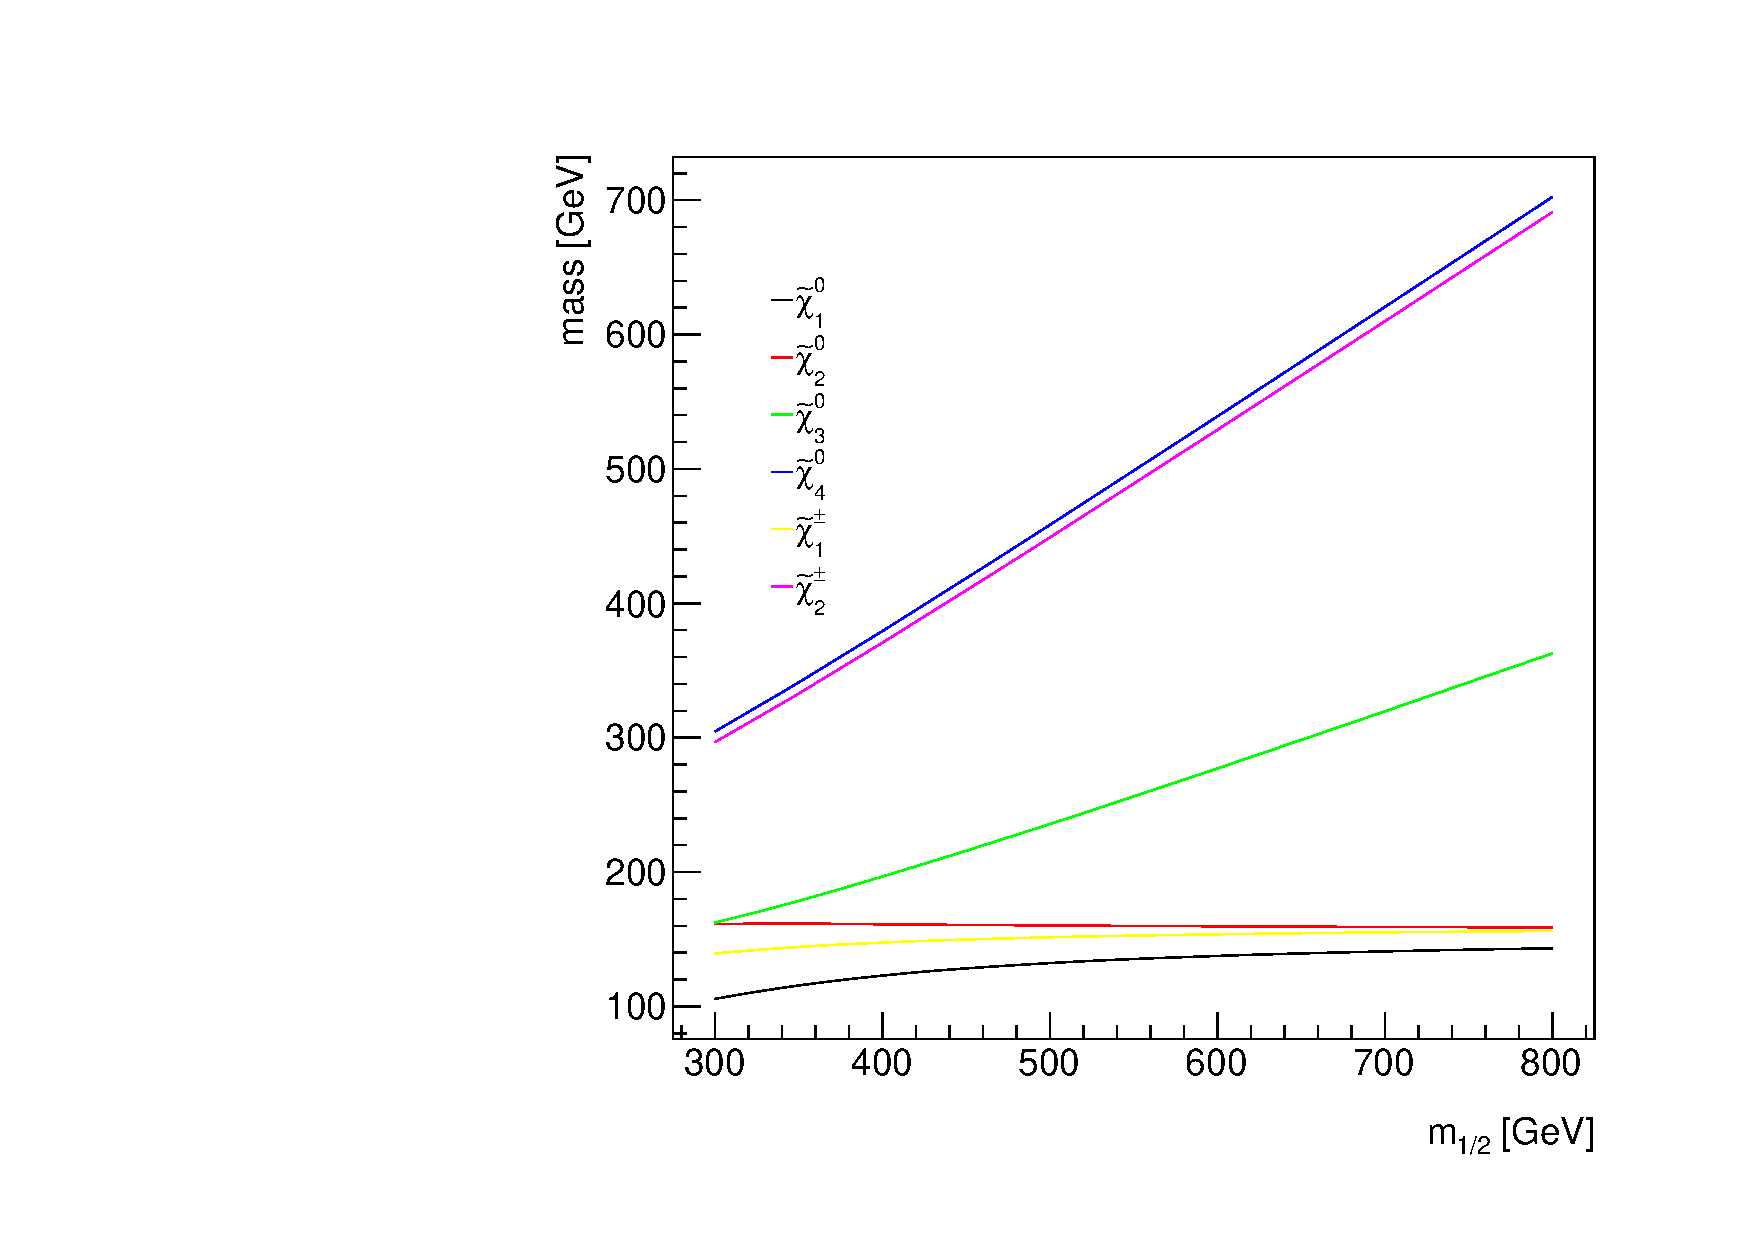
\includegraphics[scale=0.48]{mass_spectra.pdf}
        \caption{The mass spectra of the charginos $\widetilde{\chi}^{\pm}_{1,2}$ and neutralinos $\widetilde{\chi}^{0}_{1,2,3,4}$ as a function of $m_{1/2}$ in the NUHM2 model.
        The $m_{\widetilde{\chi}^{0}_{1}}$, $m_{\widetilde{\chi}^{0}_{2}}$, and $m_{\widetilde{\chi}^{\pm}_{1}}$ are roughly flat when $m_{1/2} > 500$~{\GeV}.
        The $m_{\widetilde{\chi}^{0}_{3}}$, $m_{\widetilde{\chi}^{0}_{4}}$, and $m_{\widetilde{\chi}^{\pm}_{2}}$ are heavier and increase with $m_{1/2}$.}
        \label{fig:data_mass_spectra}
    \end{center}
\end{figure}

\begin{figure}[htbp]
    \begin{center}
        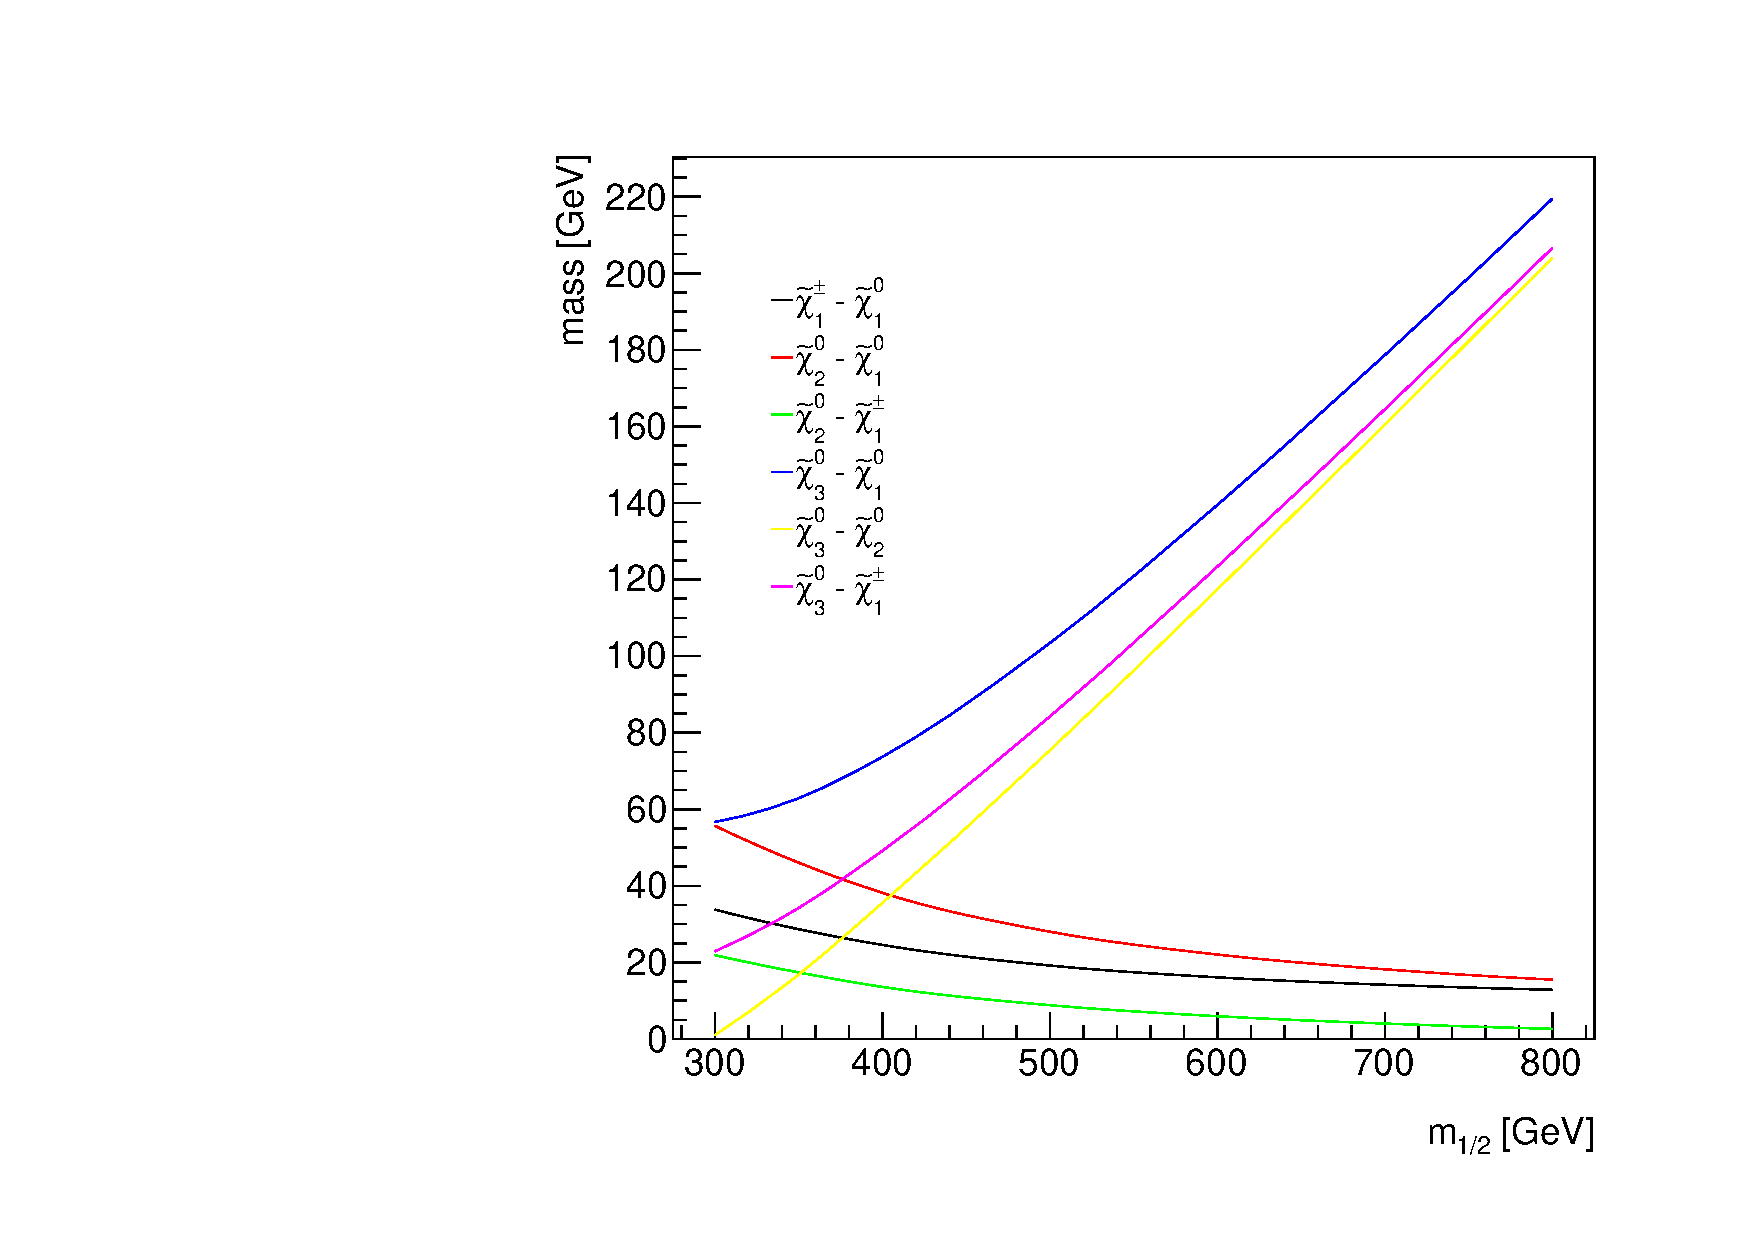
\includegraphics[scale=0.48]{mass_difference.pdf}
        \caption{The mass splitting spectra between charginos and neutralinos in the NUHM2 model.
        The mass differences $\Delta m(\widetilde{\chi}^{0}_{3}, \widetilde{\chi}^{0}_{1,2})$ and $\Delta m(\widetilde{\chi}^{0}_{3}, \widetilde{\chi}^{\pm}_{1})$ increase with $m_{1/2}$.
        The mass differences $\Delta m(\widetilde{\chi}^{\pm}_{1}, \widetilde{\chi}^{0}_{1})$, $\Delta m(\widetilde{\chi}^{0}_{2}, \widetilde{\chi}^{0}_{1})$, and $\Delta m(\widetilde{\chi}^{0}_{2}, \widetilde{\chi}^{\pm}_{1})$ decrease with $m_{1/2}$.}
        \label{fig:data_mass_splitting_spectra}
    \end{center}
\end{figure}

\begin{table}[htp]
    \begin{center}
        {\footnotesize
            \begin{tabular}{clllc}
                \hline
                \hline
                $m_{1/2}$~[{\GeV}] & $m_{\widetilde{\chi}^{0}_{2}}$~[{\GeV}] & $m_{\widetilde{\chi}^{\pm}_{1}}$~[{\GeV}] & $m_{\widetilde{\chi}^{0}_{1}}$~[{\GeV}] & ($m_{\widetilde{\chi}^{0}_{2}} - m_{\widetilde{\chi}^{\pm}_{1}}$)/($m_{\widetilde{\chi}^{\pm}_{1}} -    m_{\widetilde{\chi}^{0}_{1}}$)\\
                \hline
                350 & 161.68 & 144.29 & 115.62 & 1.61\\
                400 & 161.14 & 147.54 & 122.97 & 1.55\\
                500 & 160.30 & 151.47 & 132.28 & 1.46\\
                600 & 159.66 & 153.71 & 137.61 & 1.37\\
                700 & 159.17 & 155.14 & 140.98 & 1.28\\
                800 & 158.78 & 156.14 & 143.29 & 1.21\\
                \hline
                \hline
            \end{tabular}
        }
    \end{center}
    \caption{The masses of $\widetilde{\chi}^{0}_{1}$, $\widetilde{\chi}^{0}_{2}$, and $\widetilde{\chi}^{\pm}_{1}$ and the ratios of the mass difference between ($m_{\widetilde{\chi}^{0}_{2}} - m_{\widetilde{\chi}^{\pm}_{1}}$) and ($m_{\widetilde{\chi}^{\pm}_{1}} - m_{\widetilde{\chi}^{0}_{1}}$).
    The $m_{\widetilde{\chi}^{\pm}_{1}}$ doesn't set to the middle between $m_{\widetilde{\chi}^{0}_{1}}$ and $m_{\widetilde{\chi}^{0}_{2}}$.}
    \label{tab:data_mass_splitting_ratio}
\end{table}%

%%%
%%%
%%%

\subsubsection{The NUHM2 cross-sections}
\label{subsubsed:data_NUHM2_cross_sections}
The electroweakinos are divided into two categories, compressed and accessible, in the NUHM2 model.
The compressed category contains the lower mass charginos $\widetilde{\chi}^{\pm}_{1}$ and neutralinos $\widetilde{\chi}^{0}_{1,2}$ and the accessible category contains the higher mass charginos $\widetilde{\chi}^{\pm}_{2}$ and neutralinos $\widetilde{\chi}^{0}_{3,4}$.
Figures~\ref{fig:data_NUHM2_cross_sections_individual_and_total} shows the cross-sections for different combinations of electroweakino production and the detail values can be found in App.~\ref{app:cross_sections}.
The largest cross-section is the compressed + compressed production\footnote{Compressed + compressed means two particles belong to compressed category.} and is almost independent of $m_{1/2}$.
The cross-section of compressed + accessible\footnote{Compressed + accessible means one particle belongs to compressed category and another particle belongs to accessible.} and accessible + accessible\footnote{Accessible + accessible means two particles belong to accessible category.} productions are much smaller than the compressed + compressed production and they decrease quickly when $m_{1/2}$ increases.
Therefore, only the different combinations of compressed production are considered in this analysis.
The compressed + compressed production has cross-section about pb scale at 13~{\TeV}, hence the Higgsino analysis is expected to have good sensitivity for NUHM2 model.

\begin{figure}[htbp]
    \begin{center}
        \begin{subfigure}[b]{0.48\textwidth}
            \begin{center}
                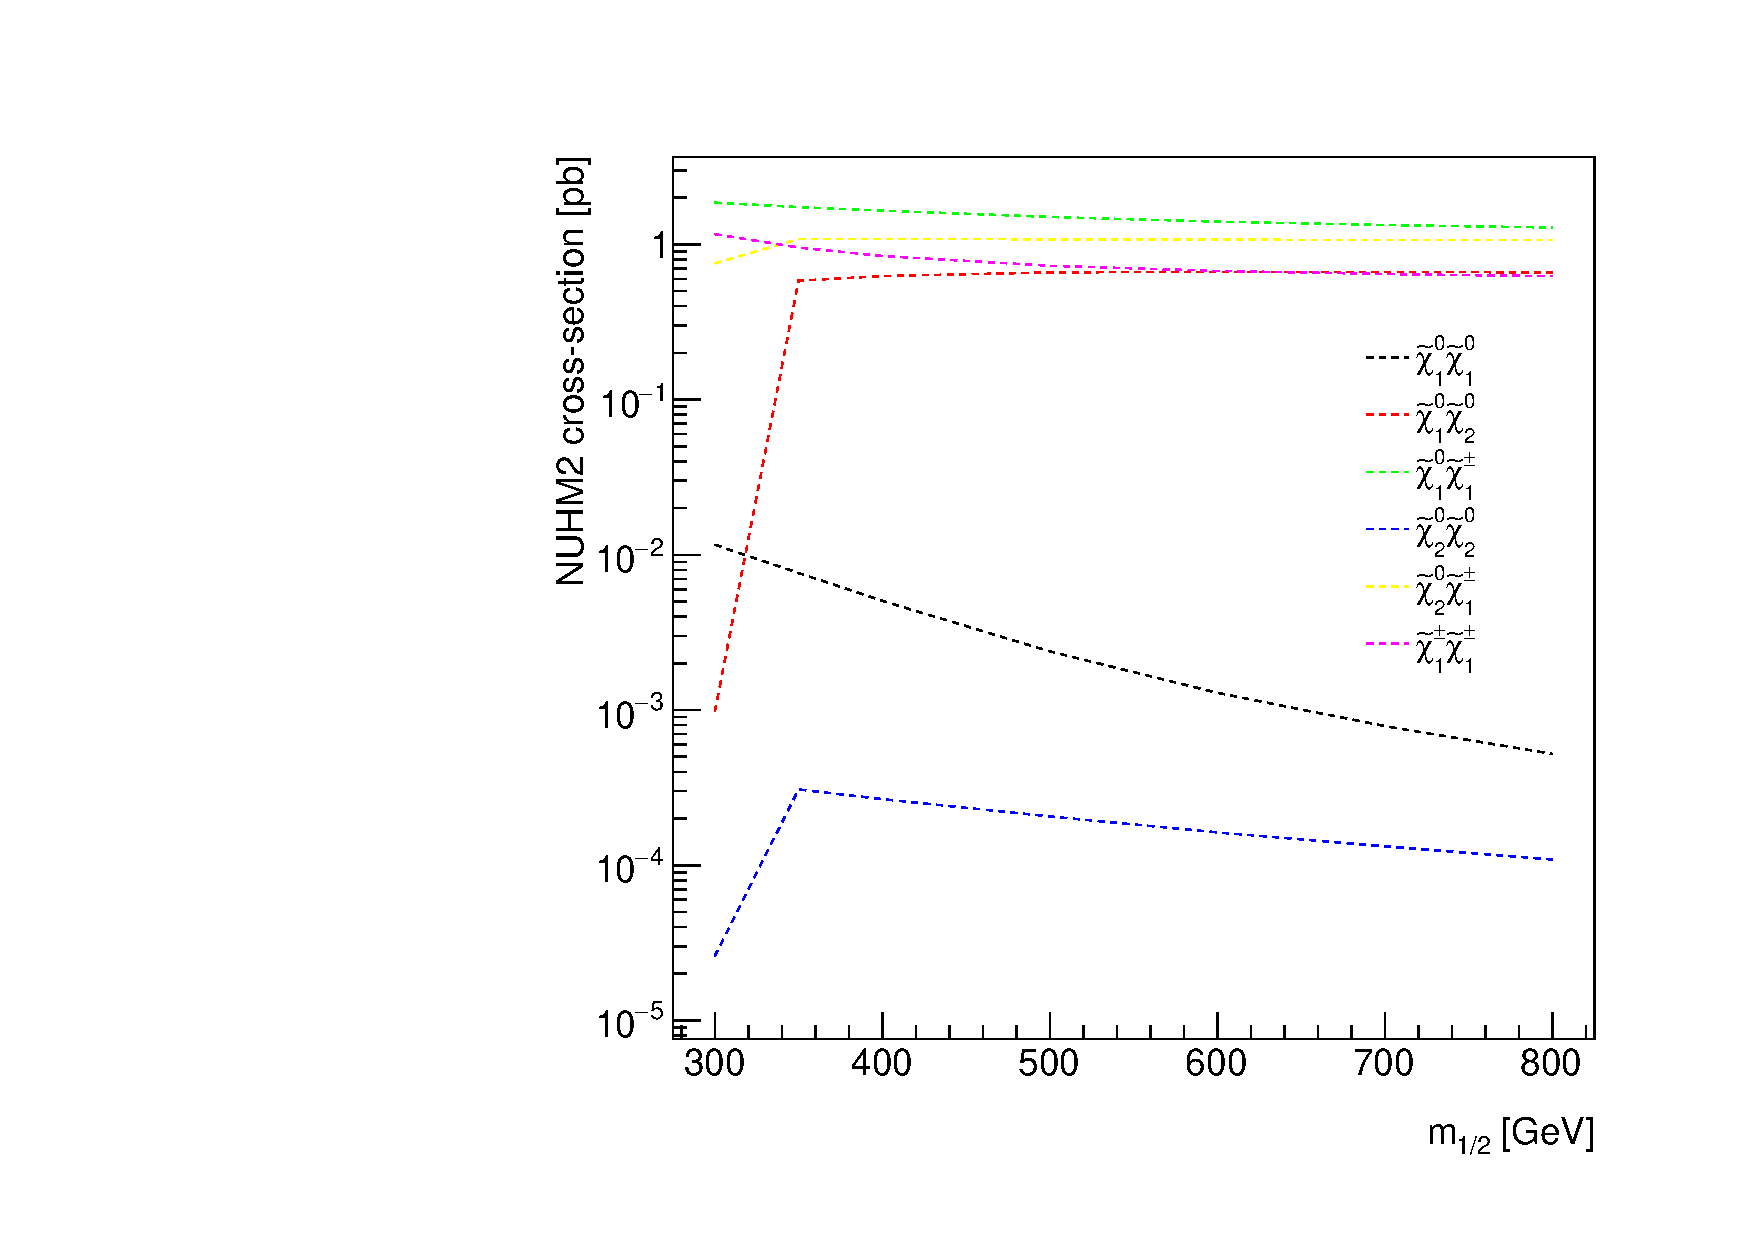
\includegraphics[scale=0.35]{Xsec_weak_individual.pdf}
                \caption{}
                \label{fig:data_NUHM2_cross_sections_individual}
            \end{center}
        \end{subfigure}%
        \begin{subfigure}[b]{0.48\textwidth}
            \begin{center}
                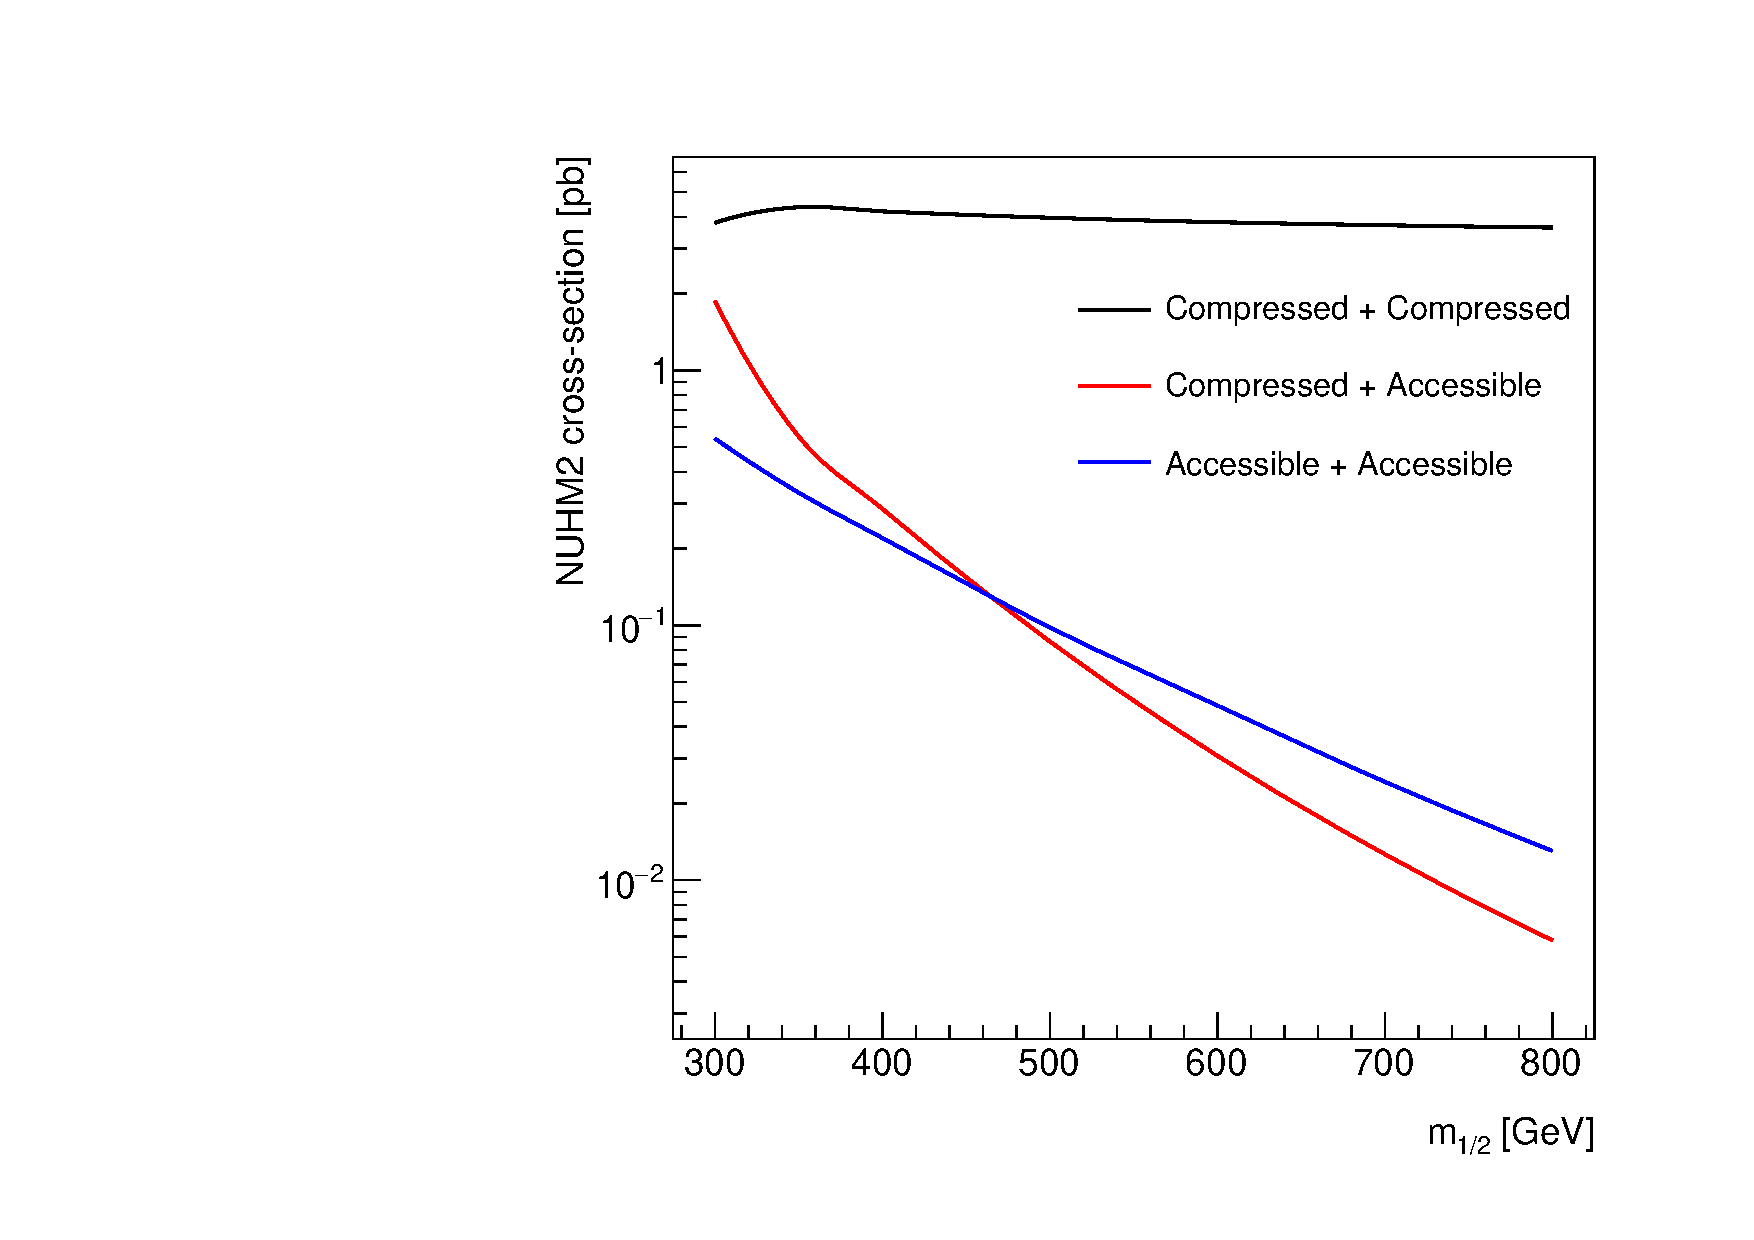
\includegraphics[scale=0.35]{Xsec_weak.pdf}
                \caption{}
                \label{fig:data_NUHM2_cross_sections}
            \end{center}
        \end{subfigure}
    \end{center}
    \caption{The NUHM2 cross-sections for (a) different combinations of compressed + compressed production and (b) all compressed + compressed, compressed + accessible, and accessible + accessible productions.}
    \label{fig:data_NUHM2_cross_sections_individual_and_total}
\end{figure}

%%%
%%%
%%%

\subsubsection{The NUHM2 production channels and relevant decays}
\label{subsubsec:data_channels_and_decays}
The compressed category contains $\widetilde{\chi}^{\pm}_{1}$, $\widetilde{\chi}^{0}_{1}$, and $\widetilde{\chi}^{0}_{2}$.
Therefore, the compressed + compressed productions can be specified by $\widetilde{\chi}^{0}_{1} \widetilde{\chi}^{0}_{1}$, $\widetilde{\chi}^{0}_{1} \widetilde{\chi}^{0}_{2}$, $\widetilde{\chi}^{0}_{1} \widetilde{\chi}^{\pm}_{1}$, $\widetilde{\chi}^{0}_{2} \widetilde{\chi}^{0}_{2}$, $\widetilde{\chi}^{0}_{2} \widetilde{\chi}^{\pm}_{1}$, and $\widetilde{\chi}^{\pm}_{1} \widetilde{\chi}^{\mp}_{1}$.
Because the highest sensitivity of this analysis is expected using two leptons, only the productions which can lead to events with two leptons are considered.
The $R$-parity conservation requires $\widetilde{\chi}^{0}_{1}$, which is LSP, to be stable, therefore, the $\widetilde{\chi}^{0}_{1} \widetilde{\chi}^{0}_{1}$ production cannot lead to events with two leptons requirement.
The cross-section of $\widetilde{\chi}^{0}_{2} \widetilde{\chi}^{0}_{2}$ production is very small so it can be neglected.
The $\widetilde{\chi}^{\pm}_{1}$ decays into a $W^{\pm}$ and a $\widetilde{\chi}^{0}_{1}$, therefore, the $\widetilde{\chi}^{0}_{1} \widetilde{\chi}^{\pm}_{1}$ production does not lead to two leptons in the final state.
Only the $\widetilde{\chi}^{0}_{2} \widetilde{\chi}^{0}_{1}$, $\widetilde{\chi}^{0}_{2} \widetilde{\chi}^{\pm}_{1}$, and $\widetilde{\chi}^{\pm}_{1} \widetilde{\chi}^{\mp}_{1}$ productions are considered in this analysis.

The neutralino $\widetilde{\chi}^{0}_{2}$ can decay into $\gamma \widetilde{\chi}^{0}_{1}$, $W^{\pm} \widetilde{\chi}^{\mp}_{1}$, $q\bar{q} \widetilde{\chi}^{0}_{1}$, $\ell^{+}\ell^{-} \widetilde{\chi}^{0}_{1}$, and $\nu\bar{\nu} \widetilde{\chi}^{0}_{1}$.
Table~\ref{tab:data_NUHM2_n2_decays} lists the branching ratios for all possible $\widetilde{\chi}^{0}_{2}$ decays for $m_{1/2} = 600$~{\GeV}.
Since the $\widetilde{\chi}^{0}_{2} \to \gamma \widetilde{\chi}^{0}_{1}$ has very small branching ratio, this decay can be neglected.

\begin{table}[htbp]
    \begin{center}
        {\footnotesize
            \begin{tabular}{lll}
                \hline
                \hline
                Decay                                                                               & Branching Ratio            & type\\
                \hline
                $\widetilde{\chi}_{2}^{0} \to \gamma \widetilde{\chi}^{0}_{1}$                      & $3.917\times 10^{-3}$ & - \\
                \hline
                $\widetilde{\chi}_{2}^{0} \to \widetilde{\chi}_{1}^{-} u \bar{d}$                   & $7.456\times 10^{-4}$ & \multirow{10}{*}{$\widetilde{\chi}^{0}_{2} \to W^{\pm} \widetilde{\chi}^{\mp}_{1}$}\\
                $\widetilde{\chi}_{2}^{0} \to \widetilde{\chi}_{1}^{-} \nu_{e} e^{+}$               & $2.485\times 10^{-4}$ & \\
                $\widetilde{\chi}_{2}^{0} \to \widetilde{\chi}_{1}^{-} \nu_{\nu} \mu^{+}$           & $2.485\times 10^{-4}$ & \\
                $\widetilde{\chi}_{2}^{0} \to \widetilde{\chi}_{1}^{+} d \bar{u}$                   & $7.456\times 10^{-4}$ & \\
                $\widetilde{\chi}_{2}^{0} \to \widetilde{\chi}_{1}^{+} e^{-} \bar{\nu}_{e}$         & $2.485\times 10^{-4}$ & \\
                $\widetilde{\chi}_{2}^{0} \to \widetilde{\chi}_{1}^{+} \mu^{-} \bar{\nu}_{\mu}$     & $2.485\times 10^{-4}$ & \\
                $\widetilde{\chi}_{2}^{0} \to \widetilde{\chi}_{1}^{-} c \bar{s}$                   & $7.456\times 10^{-4}$ & \\
                $\widetilde{\chi}_{2}^{0} \to \widetilde{\chi}_{1}^{-} \nu_{\tau} \tau^{+}$         & $2.485\times 10^{-4}$ & \\
                $\widetilde{\chi}_{2}^{0} \to \widetilde{\chi}_{1}^{+} s \bar{c}$                   & $7.456\times 10^{-4}$ & \\
                $\widetilde{\chi}_{2}^{0} \to \widetilde{\chi}_{1}^{+} \tau^{-} \bar{\nu}_{\tau}$   & $2.485\times 10^{-4}$ & \\
                \hline
                % $\widetilde{\chi}_{2}^{0} \to \widetilde{\chi}_{1}^{0} u \bar{u}$                   & $1.255\times 10^{-1}$ & \multirow{5}{*}{$\widetilde{\chi}^{0}_{2} \to q \bar{q} \widetilde{\chi}^{0}_{1}$}\\
                % $\widetilde{\chi}_{2}^{0} \to \widetilde{\chi}_{1}^{0} d \bar{d}$                   & $1.619\times 10^{-1}$ & \\
                % $\widetilde{\chi}_{2}^{0} \to \widetilde{\chi}_{1}^{0} s \bar{s}$                   & $1.619\times 10^{-1}$ & \\
                % $\widetilde{\chi}_{2}^{0} \to \widetilde{\chi}_{1}^{0} c \bar{c}$                   & $1.255\times 10^{-1}$ & \\
                % $\widetilde{\chi}_{2}^{0} \to \widetilde{\chi}_{1}^{0} b \bar{b}$                   & $9.059\times 10^{-2}$ & \\
                $\widetilde{\chi}_{2}^{0} \to \widetilde{\chi}_{1}^{0} u \bar{u}$                   & 0.126                 & \multirow{5}{*}{$\widetilde{\chi}^{0}_{2} \to q \bar{q} \widetilde{\chi}^{0}_{1}$}\\
                $\widetilde{\chi}_{2}^{0} \to \widetilde{\chi}_{1}^{0} d \bar{d}$                   & 0.162                 & \\
                $\widetilde{\chi}_{2}^{0} \to \widetilde{\chi}_{1}^{0} s \bar{s}$                   & 0.162                 & \\
                $\widetilde{\chi}_{2}^{0} \to \widetilde{\chi}_{1}^{0} c \bar{c}$                   & 0.126                 & \\
                $\widetilde{\chi}_{2}^{0} \to \widetilde{\chi}_{1}^{0} b \bar{b}$                   & 0.091                 & \\
                \hline
                $\widetilde{\chi}_{2}^{0} \to \widetilde{\chi}_{1}^{0} e^{-} e^{+}$                 & $3.672\times 10^{-2}$ & \multirow{3}{*}{$\widetilde{\chi}^{0}_{2} \to \ell^{+} \ell^{-} \widetilde{\chi}^{0}_{1}$}\\
                $\widetilde{\chi}_{2}^{0} \to \widetilde{\chi}_{1}^{0} \mu^{-} \mu^{+}$             & $3.672\times 10^{-2}$ & \\
                $\widetilde{\chi}_{2}^{0} \to \widetilde{\chi}_{1}^{0} \tau^{-} \tau^{+}$           & $3.354\times 10^{-2}$ & \\
                \hline
                $\widetilde{\chi}_{2}^{0} \to \widetilde{\chi}_{1}^{0} \nu_{e} \bar{\nu}_{e}$       & $7.307\times 10^{-2}$ & \multirow{3}{*}{$\widetilde{\chi}^{0}_{2} \to \nu \bar{\nu} \widetilde{\chi}^{0}_{1}$}\\
                $\widetilde{\chi}_{2}^{0} \to \widetilde{\chi}_{1}^{0} \nu_{\mu} \bar{\nu}_{\mu}$   & $7.307\times 10^{-2}$ & \\
                $\widetilde{\chi}_{2}^{0} \to \widetilde{\chi}_{1}^{0} \nu_{\tau} \bar{\nu}_{\tau}$ & $7.307\times 10^{-2}$ & \\
                \hline
                \hline
            \end{tabular}
        }
    \end{center}
    \caption{The possible $\widetilde{\chi}^{0}_{2}$ decays in NUHM2 model with $m_{1/2}=600$~{\GeV}.
    The $\widetilde{\chi}_{2}^{0} \to \gamma \widetilde{\chi}^{0}_{1}$ has the lowest branching ratio hence it is not considered in our study.
    The rest of the decays are categorized into 4 types as shown in the third column.}
    \label{tab:data_NUHM2_n2_decays}
\end{table}%
% \begin{table}[htbp]
%     \begin{center}
%         {\footnotesize
%             \begin{tabular}{lll}
%                 \hline
%                 \hline
%                 Decay                                                                               & Branching Ratio            & type\\
%                 \hline
%                 $\widetilde{\chi}_{2}^{0} \to \gamma \widetilde{\chi}^{0}_{1}$                      & $3.91677720\times 10^{-3}$ & - \\
%                 \hline
%                 $\widetilde{\chi}_{2}^{0} \to \widetilde{\chi}_{1}^{-} u \bar{d}$                   & $7.45565048\times 10^{-4}$ & \multirow{10}{*}{$\widetilde{\chi}^{0}_{2} \to W^{\pm} \widetilde{\chi}^{\mp}_{1}$}\\
%                 $\widetilde{\chi}_{2}^{0} \to \widetilde{\chi}_{1}^{-} \nu_{e} e^{+}$               & $2.48521683\times 10^{-4}$ & \\
%                 $\widetilde{\chi}_{2}^{0} \to \widetilde{\chi}_{1}^{-} \nu_{\nu} \mu^{+}$           & $2.48521683\times 10^{-4}$ & \\
%                 $\widetilde{\chi}_{2}^{0} \to \widetilde{\chi}_{1}^{+} d \bar{u}$                   & $7.45565048\times 10^{-4}$ & \\
%                 $\widetilde{\chi}_{2}^{0} \to \widetilde{\chi}_{1}^{+} e^{-} \bar{\nu}_{e}$         & $2.48521683\times 10^{-4}$ & \\
%                 $\widetilde{\chi}_{2}^{0} \to \widetilde{\chi}_{1}^{+} \mu^{-} \bar{\nu}_{\mu}$     & $2.48521683\times 10^{-4}$ & \\
%                 $\widetilde{\chi}_{2}^{0} \to \widetilde{\chi}_{1}^{-} c \bar{s}$                   & $7.45565048\times 10^{-4}$ & \\
%                 $\widetilde{\chi}_{2}^{0} \to \widetilde{\chi}_{1}^{-} \nu_{\tau} \tau^{+}$         & $2.48521683\times 10^{-4}$ & \\
%                 $\widetilde{\chi}_{2}^{0} \to \widetilde{\chi}_{1}^{+} s \bar{c}$                   & $7.45565048\times 10^{-4}$ & \\
%                 $\widetilde{\chi}_{2}^{0} \to \widetilde{\chi}_{1}^{+} \tau^{-} \bar{\nu}_{\tau}$   & $2.48521683\times 10^{-4}$ & \\
%                 \hline
%                 $\widetilde{\chi}_{2}^{0} \to \widetilde{\chi}_{1}^{0} u \bar{u}$                   & $1.25538409\times 10^{-1}$ & \multirow{5}{*}{$\widetilde{\chi}^{0}_{2} \to q \bar{q} \widetilde{\chi}^{0}_{1}$}\\
%                 $\widetilde{\chi}_{2}^{0} \to \widetilde{\chi}_{1}^{0} d \bar{d}$                   & $1.61880091\times 10^{-1}$ & \\
%                 $\widetilde{\chi}_{2}^{0} \to \widetilde{\chi}_{1}^{0} s \bar{s}$                   & $1.61880091\times 10^{-1}$ & \\
%                 $\widetilde{\chi}_{2}^{0} \to \widetilde{\chi}_{1}^{0} c \bar{c}$                   & $1.25538409\times 10^{-1}$ & \\
%                 $\widetilde{\chi}_{2}^{0} \to \widetilde{\chi}_{1}^{0} b \bar{b}$                   & $9.05863643\times 10^{-2}$ & \\
%                 \hline
%                 $\widetilde{\chi}_{2}^{0} \to \widetilde{\chi}_{1}^{0} e^{-} e^{+}$                 & $3.67224030\times 10^{-2}$ & \multirow{3}{*}{$\widetilde{\chi}^{0}_{2} \to \ell^{+} \ell^{-} \widetilde{\chi}^{0}_{1}$}\\
%                 $\widetilde{\chi}_{2}^{0} \to \widetilde{\chi}_{1}^{0} \mu^{-} \mu^{+}$             & $3.67224030\times 10^{-2}$ & \\
%                 $\widetilde{\chi}_{2}^{0} \to \widetilde{\chi}_{1}^{0} \tau^{-} \tau^{+}$           & $3.35381366\times 10^{-2}$ & \\
%                 \hline
%                 $\widetilde{\chi}_{2}^{0} \to \widetilde{\chi}_{1}^{0} \nu_{e} \bar{\nu}_{e}$       & $7.30678439\times 10^{-2}$ & \multirow{3}{*}{$\widetilde{\chi}^{0}_{2} \to \nu \bar{\nu} \widetilde{\chi}^{0}_{1}$}\\
%                 $\widetilde{\chi}_{2}^{0} \to \widetilde{\chi}_{1}^{0} \nu_{\mu} \bar{\nu}_{\mu}$   & $7.30678439\times 10^{-2}$ & \\
%                 $\widetilde{\chi}_{2}^{0} \to \widetilde{\chi}_{1}^{0} \nu_{\tau} \bar{\nu}_{\tau}$ & $7.30678812\times 10^{-2}$ & \\
%                 \hline
%                 \hline
%             \end{tabular}
%         }
%     \end{center}
%     \caption{The possible $\widetilde{\chi}^{0}_{2}$ decays in NUHM2 model with $m_{1/2}=600$~{\GeV}.
%     The $\widetilde{\chi}_{2}^{0} \to \gamma \widetilde{\chi}^{0}_{1}$ has the lowest branching ratio hence it is not considered in our study.
%     The rest of the decays are categorized into 4 types as shown in the third column.}
%     \label{tab:data_NUHM2_n2_decays}
% \end{table}%

The MC samples for the $\widetilde{\chi}^{0}_{2} \widetilde{\chi}^{\pm}_{1}$ generated by $pp$ collisions are produced where four kinds of $\widetilde{\chi}^{0}_{2}$ decay are specified to determine the dominant one and the $\widetilde{\chi}^{\pm}_{1}$ decay is assumed to be $\widetilde{\chi}^{\pm}_{1} \to W^{\pm} \widetilde{\chi}^{0}_{1} \to f\bar{f} \widetilde{\chi}^{0}_{1}$ where $f$ and $\bar{f}$ stand for fermion and anti-fermion.
Since $\widetilde{\chi}^{0}_{2} \to q\bar{q} \widetilde{\chi}^{0}_{1}$ and $\widetilde{\chi}^{0}_{2} \to \nu\bar{\nu} \widetilde{\chi}^{0}_{1}$ do not satisfy the two leptons requirement, the $\widetilde{\chi}^{0}_{2}$ decay should be dominated by $\widetilde{\chi}^{0}_{2} \to W^{\pm} \widetilde{\chi}^{\mp}_{1}$ and $\widetilde{\chi}^{0}_{2} \to \ell^{+}\ell^{-} \widetilde{\chi}^{0}_{1}$.
Table~\ref{tab:data_nuhm2_n2_decay_efficiency_and_percentage} shows the two leptons filter efficiency for the $\widetilde{\chi}^{0}_{2}$ decays considered, the number of events in each decay type, and the contributions to the whole $\widetilde{\chi}^{0}_{2}$ decay.
Because the $\tilde{\chi}^{0}_{2} \to \ell^{+} \ell^{-} \tilde{\chi}^{0}_{1}$ contributes more than 99\%, the other three decays can be neglected.
Although $\tilde{\chi}^{0}_{2} \to q \bar{q} \tilde{\chi}^{0}_{1}$ and $\tilde{\chi}^{0}_{2} \to \nu \bar{\nu} \tilde{\chi}^{0}_{1}$ are expected to have no contribution, due to the presence of the fake leptons, there are some contributions.
This is expected, as no requirement on the truth matching was used in the selection.

\begin{table}[htb]
    \begin{center}
        {\footnotesize
            \begin{tabular}{lccccc}
                \hline
                \hline
                \multirow{3}{*}{Decay type}                                       & \multirow{3}{*}{Branching Ratio} & \multicolumn{2}{c}{Filter efficiency}                                                                                  & \multirow{3}{*}{$N_{\mathrm{event}}$} & \multirow{3}{*}{$N_{\mathrm{event}}/N_{\mathrm{total}}$}\\
                                                                                  &                                 & $p p \to \tilde{\chi}^{0}_{2} \tilde{\chi}^{+}_{1}$        & $p p \to \tilde{\chi}^{0}_{2} \tilde{\chi}^{-}_{1}$\\
                                                                                  &                                 & $ \tilde{\chi}^{+}_{1} \to f \bar{f} \tilde{\chi}^{0}_{1}$ & $\tilde{\chi}^{-}_{1} \to f \bar{f} \tilde{\chi}^{0}_{1}$\\
                \hline
                $\tilde{\chi}^{0}_{2} \to W^{\pm} \tilde{\chi}^{\mp}_{1}$         & 0.005                           & 0.117                                                      & 0.123                                                     & 1.032 & 0.377\%\\
                $\tilde{\chi}^{0}_{2} \to q \bar{q} \tilde{\chi}^{0}_{1}$         & 0.666                           & 0.029                                                      & 0.029                                                     & 0.386 & 0.141\%\\
                $\tilde{\chi}^{0}_{2} \to \ell^{+} \ell^{-} \tilde{\chi}^{0}_{1}$ & 0.108                           & 0.606                                                      & 0.620                                                     & 272.463 & 99.482\%\\
                $\tilde{\chi}^{0}_{2} \to \nu \bar{\nu} \tilde{\chi}^{0}_{1}$     & 0.220                           & 0.010                                                      & 0.010                                                     & 0 & 0.0\%\\
                \hline
                All $\tilde{\chi}^{0}_{2}$ decays                                 & 1                               & -                                                          & -                                                         & 273.881 & 100\%\\
                \hline
                \hline
            \end{tabular}
        }
    \end{center}
    \caption{The two leptons filter efficiency for 4 kinds of $\widetilde{\chi}^{0}_{2}$ decay, the number of events for each decay in $0 < m_{\ell\ell} < 50$~{\GeV}, and the contributions to the whole $\tilde{\chi}^{0}_{2}$ decay.
    The transverse momentum of two leptons are required to be greater than 2~{\GeV} and no \met requirement is applied in the filter.}
    \label{tab:data_nuhm2_n2_decay_efficiency_and_percentage}
\end{table}%
% \begin{table}[htb]
%     \begin{center}
%         {\footnotesize
%             \begin{tabular}{lccccc}
%                 \hline
%                 \hline
%                 \multirow{3}{*}{Decay type}                                       & \multirow{3}{*}{Branching Ratio} & \multicolumn{2}{c}{Filter efficiency}                                                                                  & \multirow{3}{*}{$N_{\mathrm{event}}$} & \multirow{3}{*}{$N_{\mathrm{event}}/N_{\mathrm{total}}$}\\
%                                                                                   &                                 & $p p \to \tilde{\chi}^{0}_{2} \tilde{\chi}^{+}_{1}$        & $p p \to \tilde{\chi}^{0}_{2} \tilde{\chi}^{-}_{1}$\\
%                                                                                   &                                 & $ \tilde{\chi}^{+}_{1} \to f \bar{f} \tilde{\chi}^{0}_{1}$ & $\tilde{\chi}^{-}_{1} \to f \bar{f} \tilde{\chi}^{0}_{1}$\\
%                 \hline
%                 $\tilde{\chi}^{0}_{2} \to W^{\pm} \tilde{\chi}^{\mp}_{1}$         & 0.004473                        & 0.117129                                                   & 0.123213                                                  & 1.032 & 0.377\%\\
%                 $\tilde{\chi}^{0}_{2} \to q \bar{q} \tilde{\chi}^{0}_{1}$         & 0.665423                        & 0.029174                                                   & 0.028922                                                  & 0.386 & 0.141\%\\
%                 $\tilde{\chi}^{0}_{2} \to \ell^{+} \ell^{-} \tilde{\chi}^{0}_{1}$ & 0.106983                        & 0.605510                                                   & 0.619579                                                  & 272.463 & 99.482\%\\
%                 $\tilde{\chi}^{0}_{2} \to \nu \bar{\nu} \tilde{\chi}^{0}_{1}$     & 0.219204                        & 0.009555                                                   & 0.010037                                                  & 0 & 0.0\%\\
%                 \hline
%                 All $\tilde{\chi}^{0}_{2}$ decays                                 & 1                               & -                                                          & -                                                         & 273.881 & 100\%\\
%                 \hline
%                 \hline
%             \end{tabular}
%         }
%     \end{center}
%     \caption{The two leptons filter efficiency for 4 kinds of $\widetilde{\chi}^{0}_{2}$ decay, the number of events for each decay in $0 < m_{\ell\ell} < 50$~{\GeV}, and the contributions to the whole $\tilde{\chi}^{0}_{2}$ decay.
%     The transverse momentum of two leptons are required to be greater than 2~{\GeV} and no \met requirement is applied in the filter.}
%     %The $\tilde{\chi}^{\pm}_{1}$ is assumed to decay into $f \bar{f} \tilde{\chi}^{0}_{1}$ for all types of $\tilde{\chi}^{0}_{2}$ decay.
%     %The efficiency table contains $p p \to \tilde{\chi}^{0}_{2} \tilde{\chi}^{+}_{1}$, $\tilde{\chi}^{+}_{1} \to W^{+} \tilde{\chi}^{0}_{1} \to f \bar{f} \tilde{\chi}^{0}_{1}$ and $p p \to \tilde{\chi}^{0}_{2} \tilde{\chi}^{-}_{1}$, $\tilde{\chi}^{-}_{     1} \to W^{-} \tilde{\chi}^{0}_{1} \to f \bar{f} \tilde{\chi}^{0}_{1}$.
%     \label{tab:data_nuhm2_n2_decay_efficiency_and_percentage}
% \end{table}%

Figure~\ref{fig:data_mll_distribution} shows the $m_{\ell \ell}$ distributions in the NUHM2 model with $m_{1/2} = 600$~{\GeV} and in the simplified Higgsino model with $m_{\widetilde{\chi}^{0}_{2}} = 170$~{\GeV} and $m_{\widetilde{\chi}^{0}_{1}} = 150$~{\GeV}.
In this plot, only the $\widetilde{\chi}^{0}_{2} \widetilde{\chi}^{\pm}_{1}$ production is considered and the different $\widetilde{\chi}^{0}_{2}$ decay contributions are stacked.

\begin{figure}[htbp]
    \begin{center}
        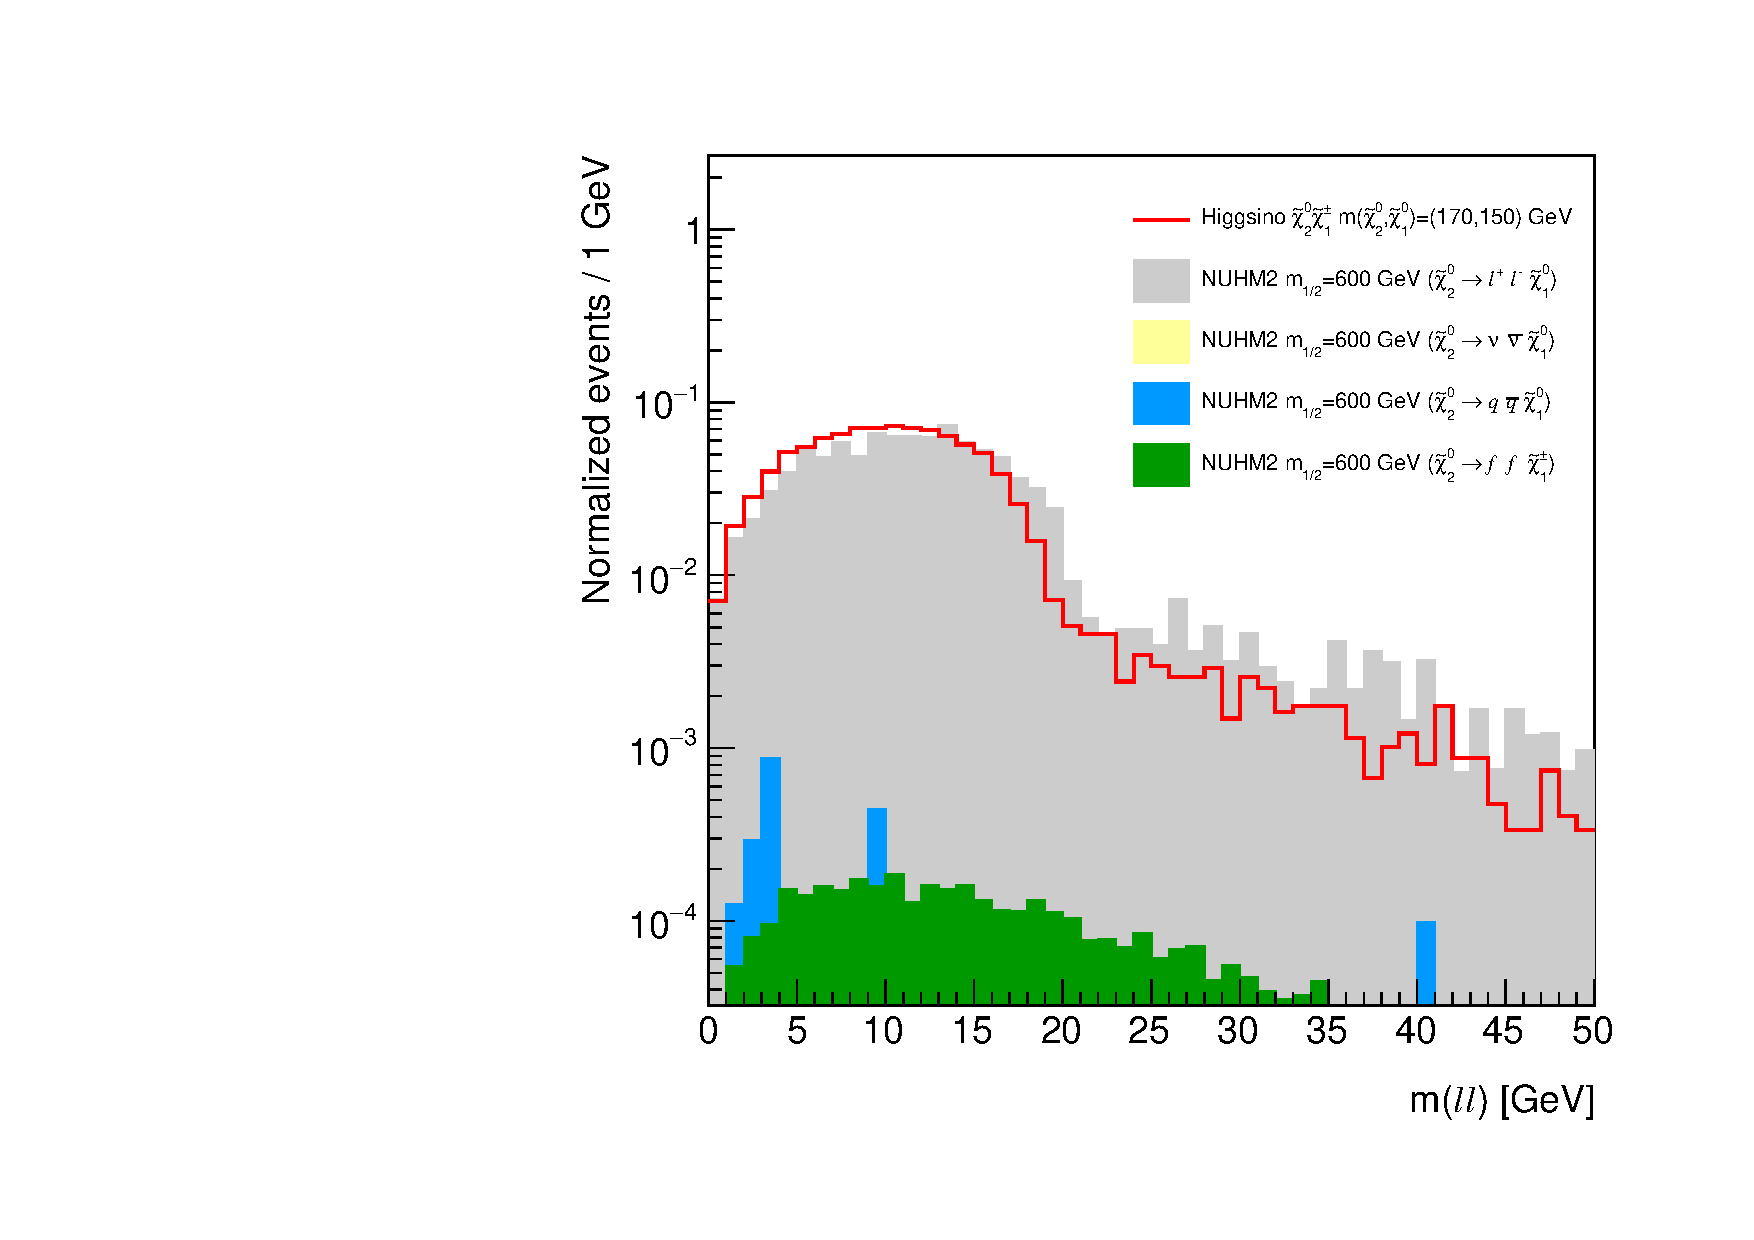
\includegraphics[scale=0.7]{mll_20171101.pdf}
        \caption{The $m_{\ell \ell}$ distributions for NUHM2 and simplified Higgsino models.
        The four possible $\widetilde{\chi}^{0}_{2}$ decay contributions for NUHM2 model are stacked and the $\widetilde{\chi}^{0}_{2} \to \ell \ell \widetilde{\chi}^{0}_{1}$ is the dominant decay (shown in grey area).
        The difference between two models come from the mass splitting $\Delta m = m_{\widetilde{\chi}^{0}_{2}} - m_{\widetilde{\chi}^{0}_{1}}$ where $\Delta m = 22$~{\GeV} for NUHM2 and $\Delta m = 20$~{\GeV} for simplified Higgsino model.}
        \label{fig:data_mll_distribution}
    \end{center}
\end{figure}

%%%
%%%
%%%

\subsubsection{The NUHM2 generation}
\label{subsubsec:data_NUHM2_generation}
The \textsc{ISAJET} 7.84 SUSY mass spectrum generator are used to calculate the NUHM2 mass spectrum.
The NUHM2 signal events were generated using MG5\_{\scriptsize A}MC@NLO v2.2.3 with NNPDF23LO PDF set up to two extra partons in the ME.
The {\MADSPIN}~\cite{Artoisenet:2012st} were used to decay the electroweakinos which were required to produce at least two leptons in the final state.
Then the results were interfaced with {\PYTHIA} v8.186 using the A14 tune to model the parton shower and hadronization.
The \textsc{Prospino} v2.1~\cite{Beenakker:1996ed} is used to calculate the cross-section and theoretical uncertainties to the next-to-leading-logarithm (NLL) level.
A filter required two leptons of at least 3~{\GeV} and \met $\ge 50$~{\GeV} was added at the generator level.
Table~\ref{tab:data_NUHM2_mcprod} lists the NUHM2 MC production samples used in this analysis.
The $\widetilde{\chi}^{0}_{2} \widetilde{\chi}^{\pm}_{1}$, $\widetilde{\chi}^{0}_{2} \widetilde{\chi}^{0}_{1}$, and $\widetilde{\chi}^{\pm}_{1} \widetilde{\chi}^{\pm}_{1}$ productions are considered in each $m_{1/2}$ mass point.
The relative branching ratios were calculated using SUSY-HIT v1.5b~\cite{Djouadi:2006bz} and were used in the event weighting.
Table~\ref{tab:data_susy_hit} compares the branching ratios for $\widetilde{\chi}^{0}_{2} \to \ell^{+} \ell^{-} \widetilde{\chi}^{0}_{1}$ and $\widetilde{\chi}^{\pm}_{1} \to \ell \bar{\nu} \widetilde{\chi}^{0}_{1}$ calculating by \textsc{ISAJET} and SUSY-HIT.
Good agreement can be seen using two different branching ratio calculators.
In the $\widetilde{\chi}^{0}_{2} \widetilde{\chi}^{\pm}_{1}$, $\widetilde{\chi}^{0}_{2} \widetilde{\chi}^{0}_{1}$ productions, the $\widetilde{\chi}^{0}_{2}$ decays via $\widetilde{\chi}^{0}_{2} \to \ell^{+} \ell^{-} \widetilde{\chi}^{0}_{1}$ and the $\widetilde{\chi}^{\pm}_{1}$ decays via $\widetilde{\chi}^{\pm}_{1} \to f\bar{f} \widetilde{\chi}^{0}_{1}$.
But in the $\widetilde{\chi}^{\pm}_{1} \widetilde{\chi}^{\mp}_{1}$ production, the $\widetilde{\chi}^{\pm}_{1}$ decays via $\widetilde{\chi}^{\pm}_{1} \to \ell \bar{\nu} \widetilde{\chi}^{0}_{1}$.

\begin{table}[htb]
    %\begin{center}
    \resizebox{\textwidth}{!}{% <------ Don't forget this %
        {\footnotesize
            \begin{tabular}{llllllll}
                \hline
                \hline
                $m_{1/2}$ [GeV] & DSID   & Production                                         & Cross-section [pb] & Process                                                                 & BF           & Filter Efficiency & Relative uncertainty\\
                \hline
                350             & 394305 & $\widetilde{\chi}^{+}_{1}\widetilde{\chi}^{-}_{1}$ & 0.9549              & $\widetilde{\chi}^{\pm}_{1} \rightarrow l \nu \widetilde{\chi}^{0}_{1}$ &  0.3333      &  0.1299           &  0.0728\\
                350             & 394306 & $\widetilde{\chi}^{0}_{2}\widetilde{\chi}^{-}_{1}$ & 0.3984              & $\widetilde{\chi}^{0}_{2} \rightarrow l l \widetilde{\chi}^{0}_{1}$     &  0.1014      &  0.2529           &  0.0860\\
                350             & 394307 & $\widetilde{\chi}^{0}_{2}\widetilde{\chi}^{+}_{1}$ & 0.6833              & $\widetilde{\chi}^{0}_{2} \rightarrow l l \widetilde{\chi}^{0}_{1}$     &  0.1014      &  0.2558           &  0.0644\\
                350             & 394308 & $\widetilde{\chi}^{0}_{2}\widetilde{\chi}^{0}_{1}$ & 0.5835              & $\widetilde{\chi}^{0}_{2} \rightarrow l l \widetilde{\chi}^{0}_{1}$     &  0.1014      &  0.2277           &  0.0719\\
                \hline
                400             & 394309 & $\widetilde{\chi}^{+}_{1}\widetilde{\chi}^{-}_{1}$ & 0.8416              & $\widetilde{\chi}^{\pm}_{1} \rightarrow l \nu \widetilde{\chi}^{0}_{1}$ &  0.3332      &  0.1220           &  0.0740\\
                400             & 394310 & $\widetilde{\chi}^{0}_{2}\widetilde{\chi}^{-}_{1}$ & 0.3977              & $\widetilde{\chi}^{0}_{2} \rightarrow l l \widetilde{\chi}^{0}_{1}$     &  0.1029      &  0.2206           &  0.0852\\
                400             & 394311 & $\widetilde{\chi}^{0}_{2}\widetilde{\chi}^{+}_{1}$ & 0.6845              & $\widetilde{\chi}^{0}_{2} \rightarrow l l \widetilde{\chi}^{0}_{1}$     &  0.1029      &  0.2239.          &  0.0648\\
                400             & 394312 & $\widetilde{\chi}^{0}_{2}\widetilde{\chi}^{0}_{1}$ & 0.6256              & $\widetilde{\chi}^{0}_{2} \rightarrow l l \widetilde{\chi}^{0}_{1}$     &  0.1029      &  0.2042           &  0.0716\\
                \hline
                500             & 394313 & $\widetilde{\chi}^{+}_{1}\widetilde{\chi}^{-}_{1}$ & 0.7281              & $\widetilde{\chi}^{\pm}_{1} \rightarrow l \nu \widetilde{\chi}^{0}_{1}$ &  0.3332      &  0.1082           &  0.0733\\
                500             & 394314 & $\widetilde{\chi}^{0}_{2}\widetilde{\chi}^{-}_{1}$ & 0.3956              & $\widetilde{\chi}^{0}_{2} \rightarrow l l \widetilde{\chi}^{0}_{1}$     &  0.1054      &  0.1892           &  0.0842\\
                500             & 394315 & $\widetilde{\chi}^{0}_{2}\widetilde{\chi}^{+}_{1}$ & 0.6819              & $\widetilde{\chi}^{0}_{2} \rightarrow l l \widetilde{\chi}^{0}_{1}$     &  0.1054      &  0.1881           &  0.0636\\
                500             & 394316 & $\widetilde{\chi}^{0}_{2}\widetilde{\chi}^{0}_{1}$ & 0.6603              & $\widetilde{\chi}^{0}_{2} \rightarrow l l \widetilde{\chi}^{0}_{1}$     &  0.1054      &  0.1760           &  0.0701\\
                \hline
                600             & 394317 & $\widetilde{\chi}^{+}_{1}\widetilde{\chi}^{-}_{1}$ & 0.6745              & $\widetilde{\chi}^{\pm}_{1} \rightarrow l \nu \widetilde{\chi}^{0}_{1}$ &  0.3332      &  0.1000           &  0.0740\\
                600             & 394318 & $\widetilde{\chi}^{0}_{2}\widetilde{\chi}^{-}_{1}$ & 0.3930              & $\widetilde{\chi}^{0}_{2} \rightarrow l l \widetilde{\chi}^{0}_{1}$     &  0.1076      &  0.1687           &  0.0834\\
                600             & 394319 & $\widetilde{\chi}^{0}_{2}\widetilde{\chi}^{+}_{1}$ & 0.6791              & $\widetilde{\chi}^{0}_{2} \rightarrow l l \widetilde{\chi}^{0}_{1}$     &  0.1076      &  0.1693           &  0.0638\\
                600             & 394320 & $\widetilde{\chi}^{0}_{2}\widetilde{\chi}^{0}_{1}$ & 0.6657              & $\widetilde{\chi}^{0}_{2} \rightarrow l l \widetilde{\chi}^{0}_{1}$     &  0.1076      &  0.1535           &  0.0705\\
                \hline
                700             & 394321 & $\widetilde{\chi}^{+}_{1}\widetilde{\chi}^{-}_{1}$ & 0.6439              & $\widetilde{\chi}^{\pm}_{1} \rightarrow l \nu \widetilde{\chi}^{0}_{1}$ &  0.3331      &  0.0935           &  0.0730\\
                700             & 394322 & $\widetilde{\chi}^{0}_{2}\widetilde{\chi}^{-}_{1}$ & 0.3913              & $\widetilde{\chi}^{0}_{2} \rightarrow l l \widetilde{\chi}^{0}_{1}$     &  0.1097      &  0.1580           &  0.0858\\
                700             & 394323 & $\widetilde{\chi}^{0}_{2}\widetilde{\chi}^{+}_{1}$ & 0.6766              & $\widetilde{\chi}^{0}_{2} \rightarrow l l \widetilde{\chi}^{0}_{1}$     &  0.1097      &  0.1587          &  0.0643\\
                700             & 394324 & $\widetilde{\chi}^{0}_{2}\widetilde{\chi}^{0}_{1}$ & 0.6643              & $\widetilde{\chi}^{0}_{2} \rightarrow l l \widetilde{\chi}^{0}_{1}$     &  0.1097      &  0.1379           &  0.0702\\
                \hline
                800             & 394325 & $\widetilde{\chi}^{+}_{1}\widetilde{\chi}^{-}_{1}$ & 0.6240              & $\widetilde{\chi}^{\pm}_{1} \rightarrow l \nu \widetilde{\chi}^{0}_{1}$ &  0.3331      &  0.0872           &  0.0724\\
                800             & 394326 & $\widetilde{\chi}^{0}_{2}\widetilde{\chi}^{-}_{1}$ & 0.3906              & $\widetilde{\chi}^{0}_{2} \rightarrow l l \widetilde{\chi}^{0}_{1}$     &  0.1116      &  0.1392           &  0.0824\\
                800             & 394327 & $\widetilde{\chi}^{0}_{2}\widetilde{\chi}^{+}_{1}$ & 0.6749              & $\widetilde{\chi}^{0}_{2} \rightarrow l l \widetilde{\chi}^{0}_{1}$     &  0.1116      &  0.1463           &  0.0628\\
                800             & 394328 & $\widetilde{\chi}^{0}_{2}\widetilde{\chi}^{0}_{1}$ & 0.6598              & $\widetilde{\chi}^{0}_{2} \rightarrow l l \widetilde{\chi}^{0}_{1}$     &  0.1116      &  0.1283           &  0.0694\\
                \hline
                \hline
            \end{tabular}
        }
    }
    %\end{center}
    \caption{The NUHM2 MC sample dataset ID (DSID), productions, cross-sections, and decay processes and its relevant branching ratios, the filter efficiencies, and the uncertainties.}
    \label{tab:data_NUHM2_mcprod}
\end{table}%
% \begin{table}[htb]
%     %\begin{center}
%     \resizebox{\textwidth}{!}{% <------ Don't forget this %
%         {\tiny
%             \begin{tabular}{llllllll}
%                 \hline
%                 \hline
%                 $m_{1/2}$ [GeV] & DSID   & Production                                         & Cross-section [pb] & Process                                                                 & BF           & Filter Efficiency & Relative uncertainty\\
%                 \hline
%                 350             & 394305 & $\widetilde{\chi}^{+}_{1}\widetilde{\chi}^{-}_{1}$ & 0.9548695995       & $\widetilde{\chi}^{\pm}_{1} \rightarrow l \nu \widetilde{\chi}^{0}_{1}$ &  0.333257248 &  0.129920         &  0.07280905\\
%                 350             & 394306 & $\widetilde{\chi}^{0}_{2}\widetilde{\chi}^{-}_{1}$ & 0.3983657446       & $\widetilde{\chi}^{0}_{2} \rightarrow l l \widetilde{\chi}^{0}_{1}$     &  0.101384714 &  0.252870         &  0.08599203\\
%                 350             & 394307 & $\widetilde{\chi}^{0}_{2}\widetilde{\chi}^{+}_{1}$ & 0.6833463531       & $\widetilde{\chi}^{0}_{2} \rightarrow l l \widetilde{\chi}^{0}_{1}$     &  0.101384714 &  0.255780         &  0.06443308\\
%                 350             & 394308 & $\widetilde{\chi}^{0}_{2}\widetilde{\chi}^{0}_{1}$ & 0.5835187445       & $\widetilde{\chi}^{0}_{2} \rightarrow l l \widetilde{\chi}^{0}_{1}$     &  0.101384714 &  0.227680         &  0.07193879\\
%                 \hline
%                 400             & 394309 & $\widetilde{\chi}^{+}_{1}\widetilde{\chi}^{-}_{1}$ & 0.8415837349       & $\widetilde{\chi}^{\pm}_{1} \rightarrow l \nu \widetilde{\chi}^{0}_{1}$ &  0.333237877 &  0.122010         &  0.07397928\\
%                 400             & 394310 & $\widetilde{\chi}^{0}_{2}\widetilde{\chi}^{-}_{1}$ & 0.3976839861       & $\widetilde{\chi}^{0}_{2} \rightarrow l l \widetilde{\chi}^{0}_{1}$     &  0.102934938 &  0.220640         &  0.08518583\\
%                 400             & 394311 & $\widetilde{\chi}^{0}_{2}\widetilde{\chi}^{+}_{1}$ & 0.6845201512       & $\widetilde{\chi}^{0}_{2} \rightarrow l l \widetilde{\chi}^{0}_{1}$     &  0.102934938 &  0.223890         &  0.06476776\\
%                 400             & 394312 & $\widetilde{\chi}^{0}_{2}\widetilde{\chi}^{0}_{1}$ & 0.6255603991       & $\widetilde{\chi}^{0}_{2} \rightarrow l l \widetilde{\chi}^{0}_{1}$     &  0.102934938 &  0.204160         &  0.07158509\\
%                 \hline
%                 500             & 394313 & $\widetilde{\chi}^{+}_{1}\widetilde{\chi}^{-}_{1}$ & 0.7280789222       & $\widetilde{\chi}^{\pm}_{1} \rightarrow l \nu \widetilde{\chi}^{0}_{1}$ &  0.333195704 &  0.108220         &  0.07328355\\
%                 500             & 394314 & $\widetilde{\chi}^{0}_{2}\widetilde{\chi}^{-}_{1}$ & 0.3955900373       & $\widetilde{\chi}^{0}_{2} \rightarrow l l \widetilde{\chi}^{0}_{1}$     &  0.105384522 &  0.189240         &  0.08416802\\
%                 500             & 394315 & $\widetilde{\chi}^{0}_{2}\widetilde{\chi}^{+}_{1}$ & 0.6819165298       & $\widetilde{\chi}^{0}_{2} \rightarrow l l \widetilde{\chi}^{0}_{1}$     &  0.105384522 &  0.188060         &  0.06356555\\
%                 500             & 394316 & $\widetilde{\chi}^{0}_{2}\widetilde{\chi}^{0}_{1}$ & 0.6603094819       & $\widetilde{\chi}^{0}_{2} \rightarrow l l \widetilde{\chi}^{0}_{1}$     &  0.105384522 &  0.176020         &  0.07005129\\
%                 \hline
%                 600             & 394317 & $\widetilde{\chi}^{+}_{1}\widetilde{\chi}^{-}_{1}$ & 0.6745140438       & $\widetilde{\chi}^{\pm}_{1} \rightarrow l \nu \widetilde{\chi}^{0}_{1}$ &  0.333158828 &  0.100020         &  0.07398616\\
%                 600             & 394318 & $\widetilde{\chi}^{0}_{2}\widetilde{\chi}^{-}_{1}$ & 0.3930396433       & $\widetilde{\chi}^{0}_{2} \rightarrow l l \widetilde{\chi}^{0}_{1}$     &  0.107603552 &  0.168710         &  0.08337329\\
%                 600             & 394319 & $\widetilde{\chi}^{0}_{2}\widetilde{\chi}^{+}_{1}$ & 0.6791453722       & $\widetilde{\chi}^{0}_{2} \rightarrow l l \widetilde{\chi}^{0}_{1}$     &  0.107603552 &  0.169260         &  0.06375124\\
%                 600             & 394320 & $\widetilde{\chi}^{0}_{2}\widetilde{\chi}^{0}_{1}$ & 0.6656504736       & $\widetilde{\chi}^{0}_{2} \rightarrow l l \widetilde{\chi}^{0}_{1}$     &  0.107603552 &  0.153530         &  0.07047924\\
%                 \hline
%                 700             & 394321 & $\widetilde{\chi}^{+}_{1}\widetilde{\chi}^{-}_{1}$ & 0.6438838471       & $\widetilde{\chi}^{\pm}_{1} \rightarrow l \nu \widetilde{\chi}^{0}_{1}$ &  0.333131205 &  0.093538         &  0.07295880\\
%                 700             & 394322 & $\widetilde{\chi}^{0}_{2}\widetilde{\chi}^{-}_{1}$ & 0.3913281838       & $\widetilde{\chi}^{0}_{2} \rightarrow l l \widetilde{\chi}^{0}_{1}$     &  0.109700775 &  0.158010         &  0.08575382\\
%                 700             & 394323 & $\widetilde{\chi}^{0}_{2}\widetilde{\chi}^{+}_{1}$ & 0.6766070496       & $\widetilde{\chi}^{0}_{2} \rightarrow l l \widetilde{\chi}^{0}_{1}$     &  0.109700775 &  0.158740         &  0.06427279\\
%                 700             & 394324 & $\widetilde{\chi}^{0}_{2}\widetilde{\chi}^{0}_{1}$ & 0.6643270342       & $\widetilde{\chi}^{0}_{2} \rightarrow l l \widetilde{\chi}^{0}_{1}$     &  0.109700775 &  0.137880         &  0.07021531\\
%                 \hline
%                 800             & 394325 & $\widetilde{\chi}^{+}_{1}\widetilde{\chi}^{-}_{1}$ & 0.6240319555       & $\widetilde{\chi}^{\pm}_{1} \rightarrow l \nu \widetilde{\chi}^{0}_{1}$ &  0.333112432 &  0.087180         &  0.07242344\\
%                 800             & 394326 & $\widetilde{\chi}^{0}_{2}\widetilde{\chi}^{-}_{1}$ & 0.3906074836       & $\widetilde{\chi}^{0}_{2} \rightarrow l l \widetilde{\chi}^{0}_{1}$     &  0.111642916 &  0.139150         &  0.08243869\\
%                 800             & 394327 & $\widetilde{\chi}^{0}_{2}\widetilde{\chi}^{+}_{1}$ & 0.6748686972       & $\widetilde{\chi}^{0}_{2} \rightarrow l l \widetilde{\chi}^{0}_{1}$     &  0.111642916 &  0.146310         &  0.06282954\\
%                 800             & 394328 & $\widetilde{\chi}^{0}_{2}\widetilde{\chi}^{0}_{1}$ & 0.6598118363       & $\widetilde{\chi}^{0}_{2} \rightarrow l l \widetilde{\chi}^{0}_{1}$     &  0.111642916 &  0.128250         &  0.06943069\\
%                 \hline
%                 \hline
%             \end{tabular}
%         }
%     }
%     %\end{center}
%     \caption{The NUHM2 MC sample dataset ID (DSID), productions, cross-sections, and decay processes and its relevant branching ratios, the filter efficiencies, and the uncertainties.}
%     \label{tab:data_NUHM2_mcprod}
% \end{table}%

\begin{table}[htb]
    \begin{center}
    %\resizebox{\textwidth}{!}{% <------ Don't forget this %
        {\footnotesize
            \begin{tabular}{clllc}
                \hline
                \hline
                $m_{1/2}$~[{\GeV}]   & Process                                                                          & \multicolumn{2}{c}{Branching ratio} & Difference (\%)\\
                                     &                                                                                  & \textsc{ISAJET} & SUSY-HIT          & \\
                \hline
                \multirow{2}{*}{350} & $\widetilde{\chi}^{\pm}_{1} \rightarrow \ell \bar{\nu} \widetilde{\chi}^{0}_{1}$ & 0.33333         & 0.33326           & 0.02\\
                                     & $\widetilde{\chi}^{0}_{2} \rightarrow \ell \ell \widetilde{\chi}^{0}_{1}$        & 0.10133         & 0.10138           & 0.05\\
                \hline
                \multirow{2}{*}{400} & $\widetilde{\chi}^{\pm}_{1} \rightarrow \ell \bar{\nu} \widetilde{\chi}^{0}_{1}$ & 0.33334         & 0.33324           & 0.03\\
                                     & $\widetilde{\chi}^{0}_{2} \rightarrow \ell \ell \widetilde{\chi}^{0}_{1}$        & 0.10288         & 0.10293           & 0.05\\
                \hline
                \multirow{2}{*}{500} & $\widetilde{\chi}^{\pm}_{1} \rightarrow \ell \bar{\nu} \widetilde{\chi}^{0}_{1}$ & 0.33334         & 0.33320           & 0.04\\
                                     & $\widetilde{\chi}^{0}_{2} \rightarrow \ell \ell \widetilde{\chi}^{0}_{1}$        & 0.10517         & 0.10538           & 0.20\\
                \hline
                \multirow{2}{*}{600} & $\widetilde{\chi}^{\pm}_{1} \rightarrow \ell \bar{\nu} \widetilde{\chi}^{0}_{1}$ & 0.33334         & 0.33316           & 0.05\\
                                     & $\widetilde{\chi}^{0}_{2} \rightarrow \ell \ell \widetilde{\chi}^{0}_{1}$        & 0.10883         & 0.10760           & 1.13\\
                \hline
                \multirow{2}{*}{700} & $\widetilde{\chi}^{\pm}_{1} \rightarrow \ell \bar{\nu} \widetilde{\chi}^{0}_{1}$ & 0.33334         & 0.33313           & 0.06\\
                                     & $\widetilde{\chi}^{0}_{2} \rightarrow \ell \ell \widetilde{\chi}^{0}_{1}$        & 0.10843         & 0.10970           & 1.16\\
                \hline
                \multirow{2}{*}{800} & $\widetilde{\chi}^{\pm}_{1} \rightarrow \ell \bar{\nu} \widetilde{\chi}^{0}_{1}$ & 0.33333         & 0.33311           & 0.07\\
                                     & $\widetilde{\chi}^{0}_{2} \rightarrow \ell \ell \widetilde{\chi}^{0}_{1}$        & 0.10947         & 0.11164           & 1.95\\
                \hline
                \hline
            \end{tabular}
        }
    %}
    \end{center}
    \caption{The branching ratios calculated by \textsc{ISAJET} and SUSY-HIT.
    The difference are calculated with respect to the SUSY-HIT branching ratio results.
    Good agreement between the results from two branching ratio calculators can be seen.
    The largest difference between the results calculating by \textsc{ISAJET} and SUSY-HIT is less than 2\%. 
    }
    \label{tab:data_susy_hit}
\end{table}%
% \begin{table}[htb]
%     \begin{center}
%     %\resizebox{\textwidth}{!}{% <------ Don't forget this %
%         {\footnotesize
%             \begin{tabular}{clllc}
%                 \hline
%                 \hline
%                 $m_{1/2}$~[{\GeV}]   & Process                                                                          & \multicolumn{2}{c}{Branching ratio} & Difference (\%)\\
%                                      &                                                                                  & \textsc{ISAJET} & SUSY-HIT          & \\
%                 \hline
%                 \multirow{2}{*}{350} & $\widetilde{\chi}^{\pm}_{1} \rightarrow \ell \bar{\nu} \widetilde{\chi}^{0}_{1}$ & 0.333335355     & 0.333257248       & 0.02\\
%                                      & $\widetilde{\chi}^{0}_{2} \rightarrow \ell \ell \widetilde{\chi}^{0}_{1}$        & 0.101330683     & 0.101384714       & 0.05\\
%                 \multirow{2}{*}{400} & $\widetilde{\chi}^{\pm}_{1} \rightarrow \ell \bar{\nu} \widetilde{\chi}^{0}_{1}$ & 0.333336010     & 0.333237877       & 0.03\\
%                                      & $\widetilde{\chi}^{0}_{2} \rightarrow \ell \ell \widetilde{\chi}^{0}_{1}$        & 0.102880344     & 0.102934938       & 0.05\\
%                 \multirow{2}{*}{500} & $\widetilde{\chi}^{\pm}_{1} \rightarrow \ell \bar{\nu} \widetilde{\chi}^{0}_{1}$ & 0.333335965     & 0.333195704       & 0.04\\
%                                      & $\widetilde{\chi}^{0}_{2} \rightarrow \ell \ell \widetilde{\chi}^{0}_{1}$        & 0.105169062     & 0.105384522       & 0.20\\
%                 \multirow{2}{*}{600} & $\widetilde{\chi}^{\pm}_{1} \rightarrow \ell \bar{\nu} \widetilde{\chi}^{0}_{1}$ & 0.333335682     & 0.333158828       & 0.05\\
%                                      & $\widetilde{\chi}^{0}_{2} \rightarrow \ell \ell \widetilde{\chi}^{0}_{1}$        & 0.108826172     & 0.107603552       & 1.13\\
%                 \multirow{2}{*}{700} & $\widetilde{\chi}^{\pm}_{1} \rightarrow \ell \bar{\nu} \widetilde{\chi}^{0}_{1}$ & 0.333335459     & 0.333131205       & 0.06\\
%                                      & $\widetilde{\chi}^{0}_{2} \rightarrow \ell \ell \widetilde{\chi}^{0}_{1}$        & 0.108425085     & 0.109700775       & 1.16\\
%                 \multirow{2}{*}{800} & $\widetilde{\chi}^{\pm}_{1} \rightarrow \ell \bar{\nu} \widetilde{\chi}^{0}_{1}$ & 0.333335274     & 0.333112432       & 0.07\\
%                                      & $\widetilde{\chi}^{0}_{2} \rightarrow \ell \ell \widetilde{\chi}^{0}_{1}$        & 0.109469250     & 0.111642916       & 1.95\\
%                 \hline
%                 \hline
%             \end{tabular}
%         }
%     %}
%     \end{center}
%     \caption{The branching ratios calculated by \textsc{ISAJET} and SUSY-HIT.
%     The difference are calculated with respect to the SUSY-HIT branching ratio results.
%     Good agreement between the results from two branching ratio calculators can be seen.
%     The largest difference between the results calculating by \textsc{ISAJET} and SUSY-HIT is less than 2\%. 
%     }
%     \label{tab:data_susy_hit}
% \end{table}%
